\documentclass[10pt]{article}
\usepackage{float}
\RequirePackage{eso-pic}
\usepackage{caption}
\captionsetup[table]{labelformat=empty}



\usepackage{geometry}
\geometry{
a4paper,
left=11mm,
right=14mm,
top=37mm,
bottom=14mm,
}



\usepackage{colortbl}
\usepackage{fontspec}
\setmainfont[Ligatures=TeX]{Calibri}



\newcommand\BackgroundPic{%
\put(0,0){%
\parbox[b][\paperheight]{\paperwidth}{%
\vfill
\centering
\includegraphics{MBIE_generic_background.pdf}%
\vfill
}}}



\begin{document}
\thispagestyle{empty}
\AddToShipoutPicture{\BackgroundPic}
\section*{Key Export Statistics\footnotemark - Peas\footnotemark }
\today\\
\begin{table}[ht]
\centering
{\scriptsize
\begin{tabular}[t]{p{1.8cm}>{\hfill}p{1.4cm}>{\hfill}p{1.4cm}>{\hfill}p{1.6cm}>{\hfill}p{1.9cm}>{\hfill}p{2cm}>{\hfill}p{1.9cm}>{\hfill}p{1.5cm}}
 \textbf{Country} & \textbf{Yearly Qty} & \textbf{Yearly Value} & \textbf{Yearly Price} & \textbf{3Year CAGR(Qty)} & \textbf{3Year CAGR(Value)} & \textbf{3Year CAGR(Price)} & \textbf{Price Elasticity} \\
\hline
Australia & 21,216 & 32.9 & \$1.5 & -0.5\% & -3.3\% & -2.8\% & 0.2 \\  
USA & 2,059 & 9.4 & \$4.6 & -10.5\% & -0.3\% & 11.4\% & -0.9 \\  
China & 5,909 & 7.9 & \$1.3 & 7.5\% & 10.9\% & 3.2\% & 2.4 \\  
Japan & 3,817 & 6.3 & \$1.7 & -3.2\% & -1.7\% & 1.6\% & -2.0 \\  
South Africa & 3,464 & 4.3 & \$1.2 & 36.9\% & 25.9\% & -8\% & -4.6 \\  
Thailand & 2,665 & 4.1 & \$1.5 & 2.1\% & 13.2\% & 10.8\% & 0.2 \\  
Other & 12,002 & 23.4 & \$1.9 & -4.8\% & 3\% & 8.2\% & -0.6 \\  
Total & 51,131 & 88.2 & \$1.7 & 0\% & 1.4\% & 1.4\% & 0.0 \\  
\hline
\end{tabular}
}
\caption{\scriptsize Top 6 Peas Markets for year ending November - 2015: Quantity('000 kg) Value(NZ\$Mill), Price and their last 3-Year Growth Rates}
\end{table}


\vspace{-0.7cm}



   \begin{figure}[H]
   \centering
    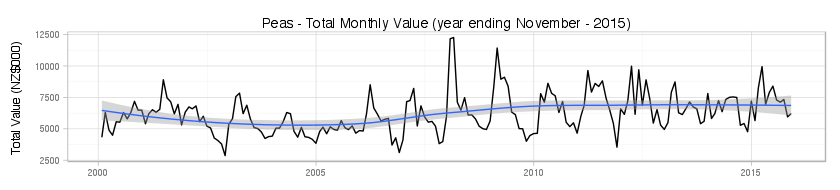
\includegraphics[scale=0.5]{../graphs/monthly_value/peas_monthly_value.png} \
    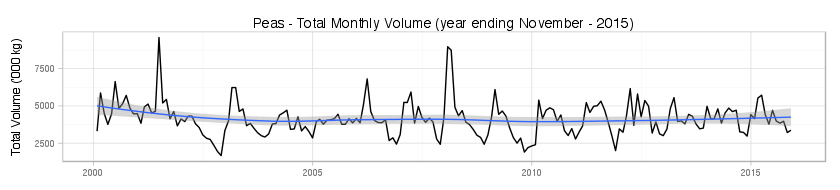
\includegraphics[scale=0.5]{../graphs/monthly_volume/peas_monthly_volume.png} \
    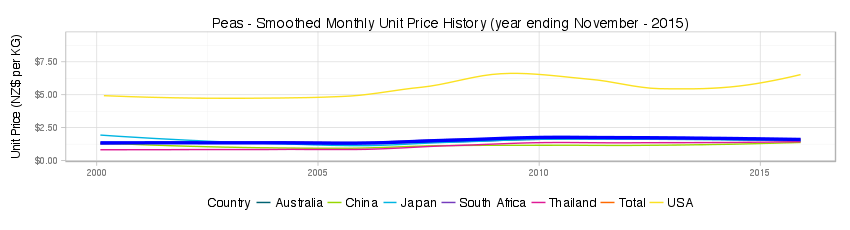
\includegraphics[scale=0.5]{../graphs/smoothed_price/peas_smoothed_price.png} \
    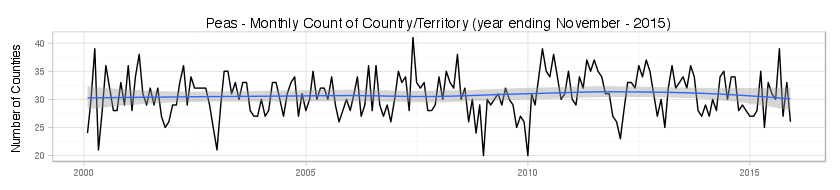
\includegraphics[scale=0.5]{../graphs/monthly_number_countries/peas_monthly_count.png} \
    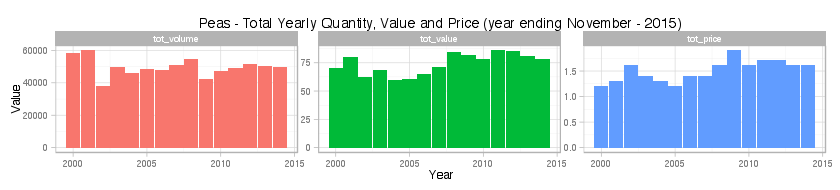
\includegraphics[scale=0.5]{../graphs/yearly_summary/peas_yearly_summary.png} \
   \end{figure}



\footnotetext[1]{Source: Statistics New Zealand - Overseas Merchandise Trade}
\footnotetext[2]{Harmonised System Codes for Peas starting with: 071021, 071310.}
\end{document}
